% Number 410
% StaticEq
% Hanging sign
% MIT

% Watermark
\AddToShipoutPicture*{\BackgroundPic}

\addtocounter {ProbNum} {1}

\begin{floatingfigure}[r]{.35\textwidth}
\includegraphics[scale=.5]{/Users/jgates/desktop/latex/pics/staticeq1.png}
\end{floatingfigure}
 
{\bf \Large{\arabic{ProbNum}}} A sign is supported by a horizontal beam and a diagonal wire as shown, both attached to a wall. The sign has a mass $m$, which is very large compared to the mass of the wire and the beam (i.e., neglect the mass of the wire and the beam). The beam pivots freely around its anchoring point in the wall, so it provides no support in the vertical direction. The angle between the wire and the beam is $\varphi$. 

\bigskip
Determine the magnitude of the force exerted by the beam.

%\begin{center}
%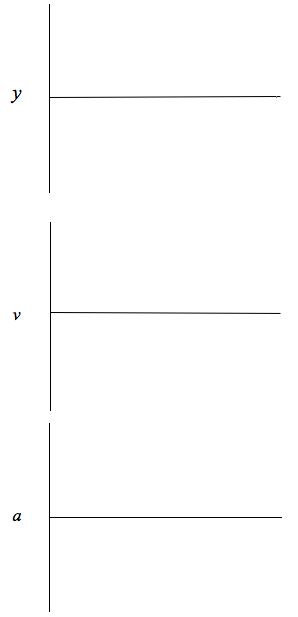
\includegraphics[scale=.85]{/Users/jgates/desktop/latex/pics/blankyvagraphstack.png}
%\end{center}


\vfill
\newpage